\documentclass[final]{beamer}
%\documentclass[10pt, handout]{beamer}
%\mode<presentation>{\usetheme{Berlin}}
%\usepackage[orientation=portrait, size=a0, scale=1.25, debug]{beamerposter}
%\documentclass[a4paper,]{article}
%\usepackage[utf8]{inputenc}
\usepackage{multicol}
%\usepackage{hyperref}
\usepackage{graphicx}
\usepackage{color}
\usepackage{framed}
\usepackage{subcaption}
\usepackage{float}
\graphicspath{ {images/} }
\usepackage{svg}
\usepackage{pdfpages}
\usepackage{blindtext}
\usepackage{mathtools}
\usepackage{amssymb}
\usepackage{amsfonts}
\usepackage{amsthm}
\usepackage[backend=biber]{biblatex}
\addbibresource{mybib.bib}
\usepackage{bm} %\bm
\usepackage{IEEEtrantools}
\usepackage[section]{placeins} %\Floatbarrier
\usepackage{float}
\usepackage{verbatim}
\usepackage{cleveref}
%\usepackage[a4paper, width=150mm, top=25mm, bottom=25mm]{geometry}
%\hypersetup{linktocpage,
%            linktoc=all,
%            %colorlinks=true,
%            %linkcolor=blue,
%}
\usepackage{lipsum}
\setlength{\parskip}{1.0em}
\setlength{\parindent}{1em}


%newcommands
\newcommand{\N}{\mathbb{N}}
\newcommand{\C}{\mathbb{C}}
\newcommand{\R}{\mathbb{R}}
%\newcommand{\Z}{\mathbb{Z}}
\newcommand{\F}{\mathbb{F}}
\newcommand{\E}{\mathbf{E}}
\newcommand{\X}{\mathbf{X}}
\newcommand{\x}{\mathbf{x}}
\newcommand{\Z}{\mathbf{Z}}
\newcommand{\z}{\mathbf{z}}
\newcommand{\Y}{\mathbf{Y}}
\newcommand{\y}{\mathbf{y}}
\newcommand{\W}{\mathbf{W}}
\newcommand{\w}{\mathbf{w}}
\newcommand{\DD}{\mathbf{D}}
\newcommand{\dd}{\mathbf{d}}
\newcommand{\LL}{\mathcal{L}}
\newcommand{\NN}{\mathcal{N}}
%\newcommand{\B}{\{-1,1\}}
%\newcommand{\bvec}[1]{\mathbf{#1}}
%\newcommand{\bv}[1]{\mathbf{#1}}
%\newcommand{\b}[1]{\boldsymbol{#1}}
\newcommand{\bv}[1]{\boldsymbol{#1}}
\newcommand{\bvec}[1]{\boldsymbol{#1}}
\newcommand{\ceil}[1]{\lceil{#1}\rceil}
\newcommand{\floor}[1]{\lfloor{#1}\rfloor}
\newcommand{\gt}{>}
\newcommand{\lt}{<}
\newcommand{\tuple}[1]{\langle #1 \rangle}

%\newcommand{\gmvaec}{$\mathrm{sc}{\ast}\mathrm{GM\Delta}$V\AE}
%\newcommand{\scgmvae}{$\mathrm{c}{\ast}\mathrm{GM\Delta}$V\AE$\mathrm{sc}$}
\newcommand{\scgmvae}{$\mathrm{c}{\ast}\mathrm{GM\Delta}$V{\AE}s---q}
%\newcommand{\gmvae}{$\mathrm{c}{\ast}\mathrm{GM\Delta}$V\AE}
\newcommand{\gmvae}{c$\ast$GM$\mathrm{\Delta}$V\AE~}

\title{\scgmvae}{}
\author{Kolb, Yiftach}
%\institute[FU and MPG]{
%  \inst{1} 
\includegraphics[width=0.3\linewidth]{images/MPIMG_RGB_gruen.png}
%  \and
%  \inst{2} 
\includegraphics[width=0.2\linewidth]{images/fu-logo_bildschirm_RGB1.jpg}
%  }
%\centering
%\vfill
%{
\includegraphics[width=0.3\linewidth]{images/MPIMG_RGB_gruen.png}} 
%{
\includegraphics[width=0.3\linewidth]{images/fu-logo_bildschirm_RGB1.jpg}}
%%\vfill
%}
%

\begin{document}
\maketitle

\section{\scgmvae}

%\begin{titlepage}
\begin{frame}
\frametitle{}
\begin{center}
{
\includegraphics[width=0.60\textwidth]{images/MPIMG_RGB_gruen.png}}\\
\vspace*{1cm}
\large
\scgmvae

\normalsize
%\large
a Master Thesis in Bioinformatics
\vspace{0.2cm}

Advisor / Reviewer: Professor Martin Vingron\\
Reviewer: Professor Tim Conrad

\vfill

%Yiftach Josef Kolb
%\normalsize{(Matrikelnummer 5195763)}

%Berlin, \today

\vfill
{
\includegraphics[width=0.4\textwidth]{images/fu-logo_bildschirm_RGB1.jpg}}
\end{center}
\normalsize
%\end{titlepage}
\end{frame}

\section{Introduction}

\begin{frame}
\frametitle{Topics to cover}
\begin{itemize}
\item{} what was our initial subject of interest
\item{} AEs are non-linear PCA basically
\item{} VAEs
\item{} other animals
\item{} GMVAE and why I derived \gmvae
\item{} example use of \gmvae on synthetic conditional-categorical data
\item{} examples on MNIST
\item{} examples on scRNAseq
\end{itemize}
\end{frame}

\begin{frame}
\frametitle{Autoencoders}

A "vanilla" autoencoder is a neural networks that "learns" the identity (subject
to dimensional restriction).

\begin{figure}[h]
%\begin{framed}
\centering
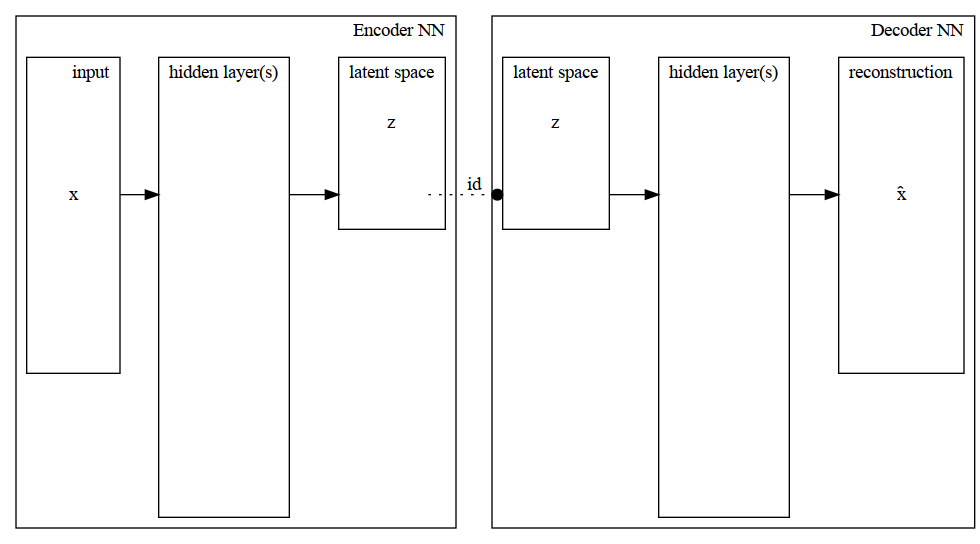
\includegraphics[width=0.9\textwidth]{./plots/autoencoderNN.gv.png}
%\label{fig:neuron1}
\caption{Autoencoder}
\label{fig:autoencoder}
%\end{framed}
\end{figure}

\end{frame}


\begin{frame}
\frametitle{Autoencoders and PCA}

(On centered data\cite{plaut2018principal})

PCA
{\small
\begin{equation}
\label{eqn:pca}
\bv{\tilde{V}} = \text{argmin}_{\W} \{
\|\X - \X \bv{W}\bv{W}^T\|_F^2 \quad : \quad \bv{W} \in \R^{n \times l}, \bv{W}^T \bv{W} =
\bv{I}_l\}
\end{equation} 
}

Linear AE
{\small
\begin{IEEEeqnarray}{C}
\label{eqn:pca2}
%\begin{aligned}
\text{argmin}_{\bv{E,D}}\{\|\X - \X \bv{E}\bv{D}\|_F^2 \quad : 
\quad \bv{E,D^T} \in \R^{n \times
l},\} \\
\label{eqn:pca3}
\bv{\tilde{W}}
\in \text{argmin}_{\W}\{\|\X - \X \bv{W}\bv{W}^{\dagger}\|_F^2 \quad : 
\quad \bv{W} \in \R^{n \times
l},\}
%\end{aligned}
\end{IEEEeqnarray}
}

$
\text{span}\{\bv{\tilde{W}}\} = \text{span}\{\bv{\tilde{V}}\}
$


\end{frame}


\begin{frame}
\frametitle{VAEs}
\begin{figure}[h]
%\begin{framed}
\centering
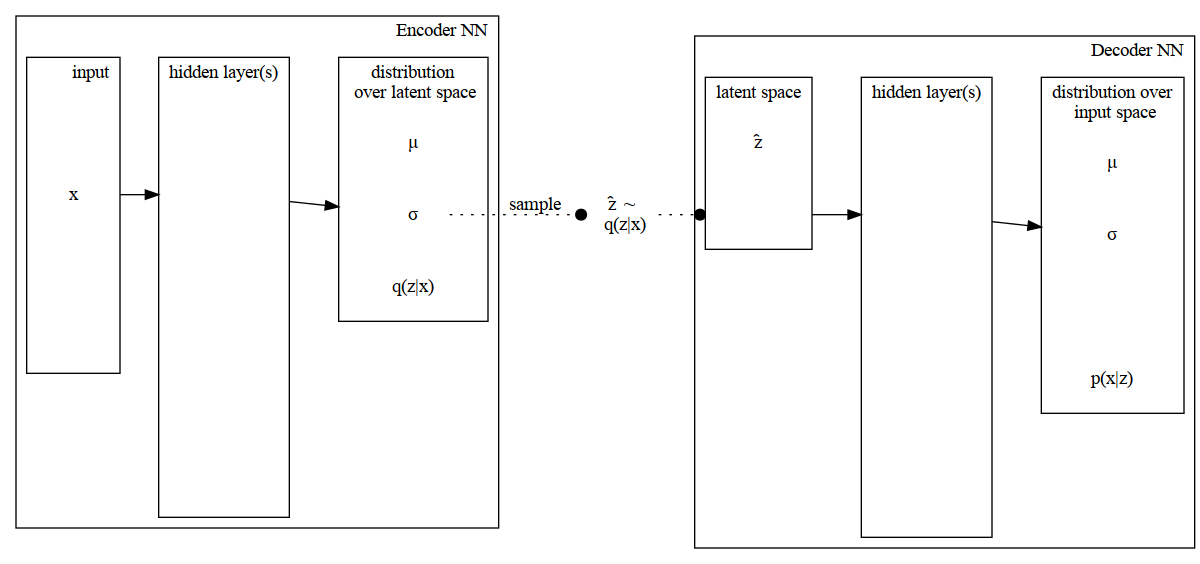
\includegraphics[width=0.99\textwidth]{./plots/vaeNN.gv.png}
%\label{fig:neuron1}
\caption{VAE}
\label{fig:vae}
%\end{framed}
\end{figure}
\end{frame}



\section{bigass equation}

\begin{frame}

{\tiny
\begin{equation}
\label{eq:elbo}
\begin{aligned}
\frac{1}{N} \log p(\bv{X}) &= \frac{1}{N} \log \int p(\bv{X},\bv{Z}) d\bv{Z} 
& \text{taking marginal} \\
& = \frac{1}{N} \log \int \frac{p(\bv{X},\bv{Z})}{q(\bv{Z})} q(\bv{Z})d\bv{Z} 
& \text{multiplying by 1 inside}\\
&=  \frac{1}{N} \log \int \frac{p(\bv{X},\bv{Z})}{q(\bv{Z})}dq(\bv{Z}) 
& \text{definition of } dq(\Z)\\
&\geq  \frac{1}{N} \int \log \frac{p(\bv{X},\bv{Z})}{q(\bv{Z})}dq(\bv{Z}) 
& \text{Jensen inequality}\\
&= \frac{1}{N} \int \sum_1^N \log \frac{p(\x_i, \z_i)}{q(\z_i)}dq(\z_i) 
& \text{using the iid property}\\
&= \frac{1}{N} \sum_1^N - \LL(q,p,\x_i)
& \text{definition of } \LL(q,p,\x_i)\\
& = -\mathcal{L}(q,p,X) \triangleq -\mathcal{L}(q,p)
& \text{again definition of } \LL(p,q) \qed
\end{aligned}
\end{equation}
}
\end{frame}

\begin{frame}
normal text
\tiny
tiny text
\normalsize
normal text
And now to something~\cite{guo2017improved} completely different \dots
\end{frame}

%\begin{frame}
%\frametitle{Spam}
%\begin{block}
%\maketitle
%\end{block}
%%\titlepage
%\begin{multicols}{2}
%Spam~\footfullcite{russkikh2020style} is good.
%spam spam spam
%\lipsum[1]
%\lipsum[2]
%\end{multicols}
%\end{frame}
%
%\begin{frame}
%\frametitle{Bigass equation}
%foo
%far
%\end{frame}

%\begin{frame}
%And now to something~\cite{guo2017improved} completely different \dots
%\end{frame}

\section{Reference}
\begin{frame}
\printbibliography
\end{frame}

\begin{comment}
\end{comment}

\end{document}
